\begin{enumerate}
  \item Definiční obor
  \item Derivace
  \item Nulové body - znaménko $^+_-$
  \item Intervaly, uzavřenost nul. bodů
    \begin{itemize}
      \item rostoucí
      \item klesající
    \end{itemize}
\end{enumerate}
\subsubsection{Monotonie - příklady}
\begin{align*}
  f(x)&=\frac{x^2}{x+2}
\end{align*}
\hrule
\begin{align*}
  f'(x)&=\frac{x*(x+4)}{(x+2)^2} \\
\end{align*}

\begin{center}
  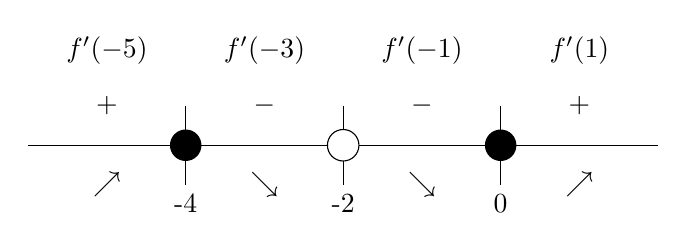
\begin{tikzpicture}[scale=1]
    \draw (-6,0)-- (2,0); %Axis
    \foreach \x in {-4,-2,0} {
      \draw (\x,0.5) -- (\x,-0.5) node[below] {\x};
    }
    \fill (-4,0) circle (0.2);
    \draw[fill=white] (-2,0) circle (0.2);
    \fill (0,0) circle (0.2);
    \draw (-5,0.5) node{$+$} (-5,-0.5) node{$\nearrow$} (-5,1.2) node{$f'(-5)$};
    \draw (-3,0.5) node{$-$} (-3,-0.5) node{$\searrow$} (-3,1.2) node{$f'(-3)$};
    \draw (-1,0.5) node{$-$} (-1,-0.5) node{$\searrow$} (-1,1.2) node{$f'(-1)$};
    \draw (1,0.5) node{$+$} (1,-0.5) node{$\nearrow$} (1,1.2) node{$f'(1)$};
  \end{tikzpicture}
\end{center}

\begin{center}
  rostoucí na $(\infty;-4\rangle \text{ a } (0;\infty)$ \\
  klesající na $\langle-4;-2) \text{ a } (-2;0\rangle$
\end{center}
